\let\negmedspace\undefined
\let\negthickspace\undefined
\documentclass[journal,12pt,onecolumn]{IEEEtran}
\usepackage{cite}
\usepackage{amsmath,amssymb,amsfonts,amsthm}
\usepackage{algorithmic}
\usepackage{graphicx}
\graphicspath{{./figs/}}
\usepackage{textcomp}
\usepackage{xcolor}
\usepackage{txfonts}
\usepackage{listings}
\usepackage{enumitem}
\usepackage{mathtools}
\usepackage{gensymb}
\usepackage{comment}
\usepackage{caption}
\usepackage[breaklinks=true]{hyperref}
\usepackage{tkz-euclide} 
\usepackage{listings}
\usepackage{gvv}                                        
%\def\inputGnumericTable{}                                 
\usepackage[latin1]{inputenc}     
\usepackage{xparse}
\usepackage{color}                                            
\usepackage{array}
\usepackage{longtable}                                       
\usepackage{calc}                                             
\usepackage{multirow}
\usepackage{multicol}
\usepackage{hhline}                                           
\usepackage{ifthen}                                           
\usepackage{lscape}
\usepackage{tabularx}
\usepackage{array}
\usepackage{float}
\newtheorem{theorem}{Theorem}[section]
\newtheorem{problem}{Problem}
\newtheorem{proposition}{Proposition}[section]
\newtheorem{lemma}{Lemma}[section]
\newtheorem{corollary}[theorem]{Corollary}
\newtheorem{example}{Example}[section]
\newtheorem{definition}[problem]{Definition}
\newcommand{\BEQA}{\begin{eqnarray}}
\newcommand{\EEQA}{\end{eqnarray}}
\newcommand{\define}{\stackrel{\triangle}{=}}
\theoremstyle{remark}
\newtheorem{rem}{Remark}

\begin{document}

\title{1.10.19}
\author{ee25btech11056 - Suraj.N}
\maketitle
\renewcommand{\thefigure}{\theenumi}
\renewcommand{\thetable}{\theenumi}

\textbf{Question} : If a line has direction ratios $2,-1,-2$, determine its direction cosines. 

\textbf{Solution} : 

\begin{table}[h!]
  \centering
  

  \caption*{Table : Vector}
  \label{1.10.19}
\end{table}

The direction vector of the line is
\begin{align*}
\vec{a} &= \myvec{2\\-1\\-2}
\end{align*}

The length of $\vec{a}$ is
\begin{align*}
a^\top a &= \myvec{2 & -1 & -2}\myvec{2\\-1\\-2} \\
&= 2^2 + \brak{-1}^2 + \brak{-2}^2 \\
&= 4 + 1 + 4 = 9
\end{align*}

Therefore, the norm of $a$ is
\begin{align*}
\norm{a} &\overset{\Delta}{=} \sqrt{a^\top a} = \sqrt{9} = 3
\end{align*} 

The unit vector in the direction of $\vec{a}$ is  

\begin{align*} 
\frac{\vec{a}}{\norm{\vec{a}}}
&= \frac{1}{3}\myvec{2\\-1\\-2}
\end{align*}

Let $\alpha,\beta,\gamma$ be the angles made by the line with the $x,y,z$ axes respectively.Then, the direction cosines are the elements of the above direction vector
\begin{align*}
\cos\alpha = \frac{2}{3}, \quad
\cos\beta = -\frac{1}{3}, \quad
\cos\gamma = -\frac{2}{3}
\end{align*}

\pagebreak

\begin{figure}[h!]
  \centering
  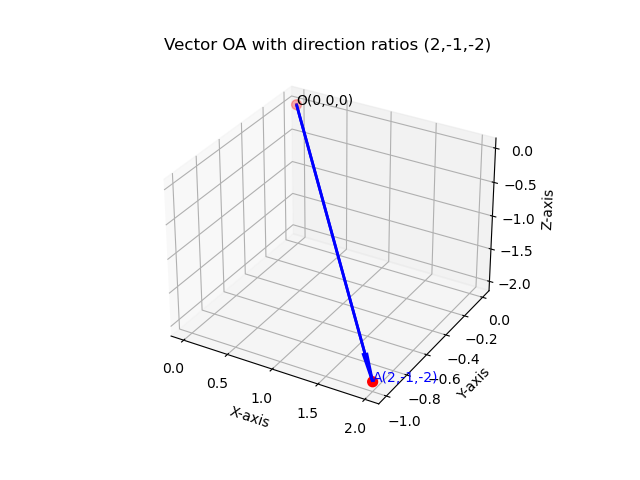
\includegraphics[width=0.9\columnwidth]{figs/fig_vector.png} 
   \caption*{Fig : Vector a}
  \label{Fig1}
\end{figure}


\end{document}











































































\end{document}
